\chapter{KDE}

\section{Introduction}

At that time, none of the application under Unix dekstop, including the desktop
itself, has a nice interface. Matthias Ettrich want to build not only a set of
applications, but a desktop environment in which users could expect things to
look, feel, and work consistently. Then, he founded KDE project in 1996. KDE
stands for K Desktop Environment, with K = Kool or Common, defined by Matthias
Ettrich. Nowadays, it's considered as the coolest or most widely used
cross-platform desktop environment.

Initially, KDE use Motif graphical widget toolkit to develop interface and
productivity tools. Then, Matthias decided to use Qt library for developing GUI
(Chap.\ref{chap:Qt}) for KDE. To guarantee Qt is availble for free with KDE, KDE
Free Qt foundation was created. [NOTE: As an effort to avoid using commercial
product like Qt, GNOME project was started in 1997]. In 1998, the first KDE/Qt
desktop environment, KDE 1.0, was released, Fig.\ref{fig:kde1}.
Many softwares used KDE have the name with 'K' as prefixes, e.g. Konsole (free
terminal emulator), Kaffeine (a media-player). The core libraries of KDE was
licensed under GNU LGPL; but proprietary software need to follow Qt properietary
license to use KDE.


In 2000, KDE 2.0 was released with major changes: KParts (allow an application
to embed another within itself), KHTML (a HTML rendering engine used by
Konqueror web browser), KIO (I/O library), DCOP (Desktop COmmunication
Protocol).

In 2002, KDE 3.0 Dekstop Environment was released, built upon Qt 3 (released
under LGPL for Linux or Unix-like OS only). To run on Windows, it need KDE on
Cygwin (which is now stopped due to available of KDE 4 fow Windows).

In 2008, KDE 4.0 Dekstop Environment was released based on Qt 4 (released under
LGPL for both Windows and MacOS X).  Since 2009, KDE projects was rebranded,
giving KDE no longer stands for K Desktop Environment, but act as an umbrella
brand for software produced by the community. So, from KDE 4.0, KDE (desktop)
was given the name KDE Software Compilation 4 (KDE SC 4) or {\bf KDE platform
4}. The term doesn't target to any particular KDE product.
So, KDE-based software like Amarok or Digikam, are not part of KDE SC. Also,
since then, no major release of KDE has been announced since the acquisition of
Trolltech (the company manage Qt) by Nokia. Major changes are:
\begin{enumerate}
  \item Kicker (the main panel like Star horizonal bar on Windows) + KDesktop
  (a virtual background window to draw icons or other graphics) +
  SuperKarambar (a tool allowing programmers to create gadgets on KDesktop
  virtual window) $\rightarrow$ they are all replaced by KDE Plasma. There are
  three workspaces: KDE Plasma Desktop, KDE Plasma Netbook and KDE Plasma
  Active (for tablet, phone). 
  
%   4.9 with different layout, e.t.
%   Dolphin
   
\end{enumerate}


Since 2011, CMake was used as the build tool for KDE, giving better support for
a wide range of platform. Roadmap for KDE 5.0 was announced in Aug, 2011
\footnote{\url{http://www.itworld.com/mobile-wireless/191083/kde-50-roadmap-announced}}.
Major changes include focusing on mobile devices

% When KDE and Qt are libraries for developing GUI, a
% common name them is {\it widget toolkit}. Qt can also be used to develop non-GUI
% applications.

\begin{figure}[hbt]
  \centerline{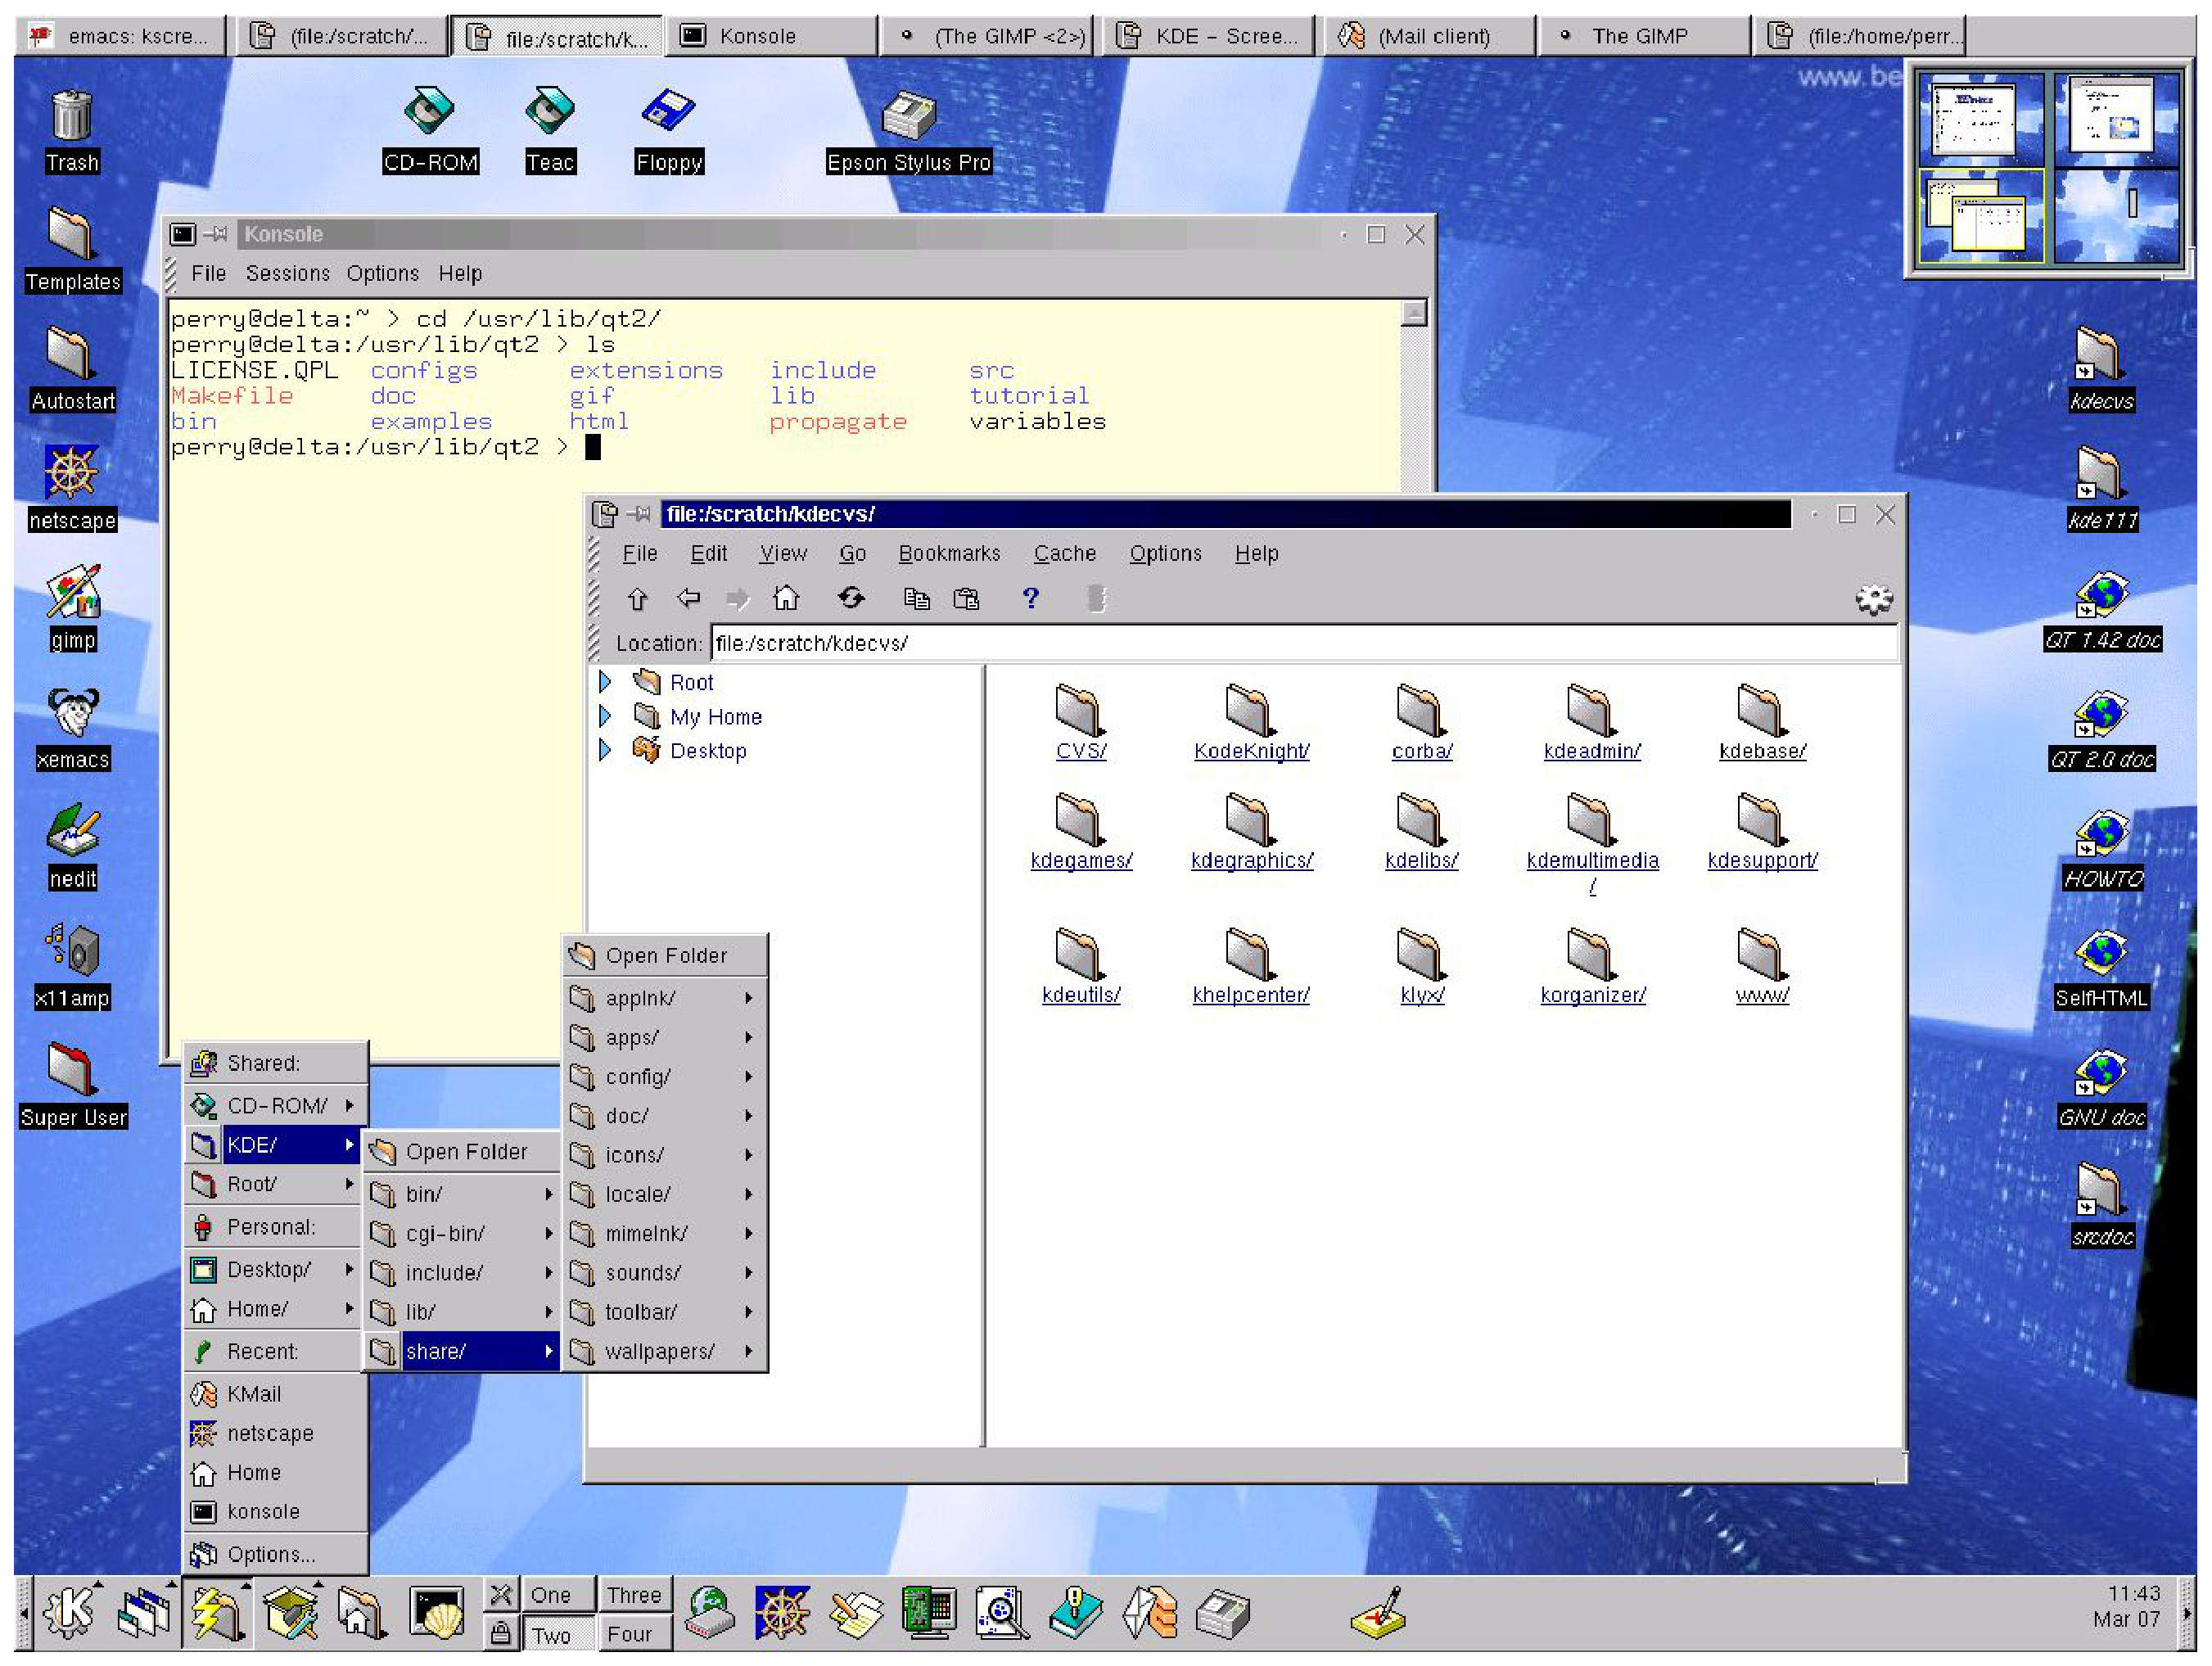
\includegraphics[height=5cm,
    angle=0]{./images/kde1.eps}}
\caption{KDE 1.0 Desktop}
\label{fig:kde1}
\end{figure}

